\section{Algoritmos de balanceamento}

\begin{frame}[fragile]{Balanceamento por inserção}

    \begin{itemize}
        \item Uma maneira de garantir o balanceamento de uma árvore binária de busca
                é utilizar um processo de
            inserção controlada, de modo que ao final das inserções a árvore resultante esteja
            balanceada

        \item Futuras inserções ou remoções podem resultar no desbalanceamento da árvore

        \item Esta estratégia é útil quando os elementos a serem inseridos são conhecidos de
            antemão e quando não haverão novas inserções ou remoções

        \item O algoritmo $O(N\log N)$ que resulta em uma árvore balanceada é
        \begin{enumerate}
            \item armazene os $N$ elementos a serem inseridos em um vetor $v$
            \item ordene $v$ em ordem crescente
            \item insira o elemento central $x$ do vetor na árvore
            \item continue o processo no subvetor à esquerda de $x$
            \item finalize o processo no subvetor à direita de $x$
        \end{enumerate}
    \end{itemize}

\end{frame}

\begin{frame}[fragile]{Algoritmo de inserção balanceada}
    \inputsnippet{cpp}{1}{21}{balanced_insertion.cpp}
\end{frame}

\begin{frame}[fragile]{Algoritmo de inserção balanceada}
    \inputsnippet{cpp}{22}{42}{balanced_insertion.cpp}
\end{frame}

\begin{frame}[fragile]{Notas sobre o algoritmo de balanceamento por inserção}

	\begin{itemize}
		\item O algoritmo proposto tem duas grandes {desvantagens}: é necessário {armazenar} os 
            elementos antes da inserção na árvore e ordenar dos elementos armazenados

		\item Se a árvore já tiver sido construída previamente, uma solução é {preencher} um vetor 
            atráves de uma travessia {em-order}, {destruir} a árvore e {reconstruí-la}

		\item A solução apresentada {remove} a necessidade de ordenamento, uma vez que a 
            travessia {em-order} garante que o vetor estará {ordenado}

        \item Outro ponto importante é que futuras inserções podem desfazer o balanceamento da árvore
	\end{itemize}

\end{frame}

\begin{frame}[fragile]{Algoritmo DSW}

	\begin{itemize}
		\item O algoritmo DSW foi proposto por {Colin Day} e melhorado por {Quentin F. Stout} e {Bete L. Warren}

		\item Ele consiste no {reposicionamento} dos nós através de operações de {rotação} do 
            filho \code{c}{C} em torno do seu pai \code{c}{P}, o que pode pode envolver seu avô 
            \code{c}{G}

		\item A rotação pode ser feita tanto para a {esquerda} quanto para a {direita}

        \item Na rotação à esquerda, o filho (inicialmente à direita do pai) passa a ocupar a 
            posição do pai, que se torna seu filho à esquerda

        \item Caso o filho tenha uma subárvore à esquerda antes da rotação, esta subárvore se
            torna o filho à direita do pai, após a rotação

        \item A rotação à direita faz processo simétrico, no sentido horário
	\end{itemize}

\end{frame}

\begin{frame}[fragile]{Implementação da rotação à esquerda}
    \inputcode{cpp}{rotate_left.cpp}
\end{frame}


\begin{frame}[fragile]{Implementação da rotação à direita}
    \inputcode{cpp}{rotate_right.cpp}
\end{frame}

\begin{frame}
\frametitle{Exemplo de rotação à direita}

    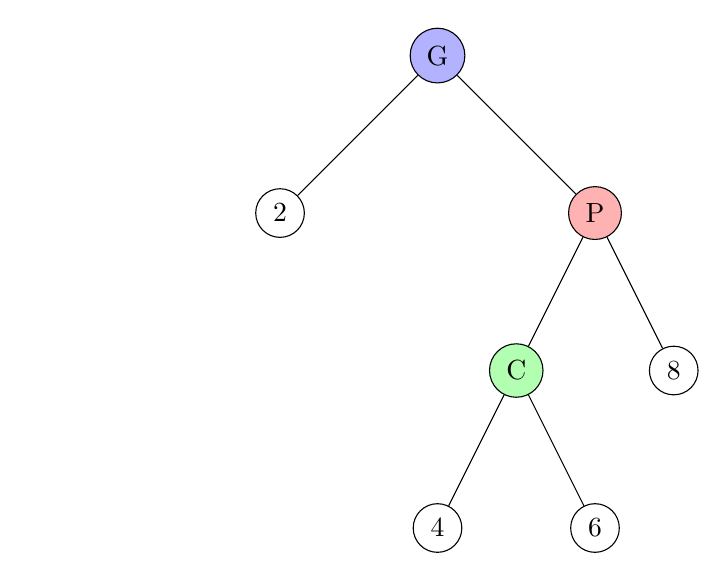
\begin{tikzpicture}
        \begin{scope}{shift={(3,0)}}
            \node[opacity=0] (X) at (-1, 2) { $1$ };
            \node[circle,draw,fill=blue!30] (A) at (4, 8) { G };
            \node[circle,draw] (B) at (2, 6) { 2 };
            \node[circle,draw,fill=red!30] (C) at (6, 6) { P };
            \node[circle,draw,fill=green!30] (D) at (5, 4) { C };
            \node[circle,draw] (E) at (7, 4) { 8 };
            \node[circle,draw] (F) at (4, 2) { 4 };
            \node[circle,draw] (G) at (6, 2) { 6 };

            \draw (A) -- (B);
            \draw (A) -- (C);
            \draw (C) -- (D);
            \draw (C) -- (E);
            \draw (D) -- (F);
            \draw (D) -- (G);
        \end{scope}
    \end{tikzpicture}

\end{frame}

\begin{frame}
\frametitle{Exemplo de rotação à direita}

    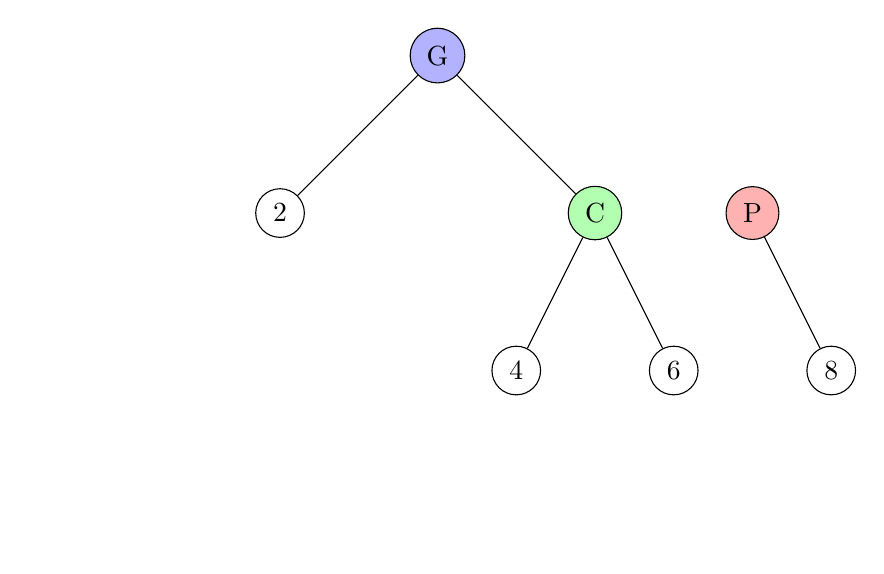
\begin{tikzpicture}
        \begin{scope}{shift={(3,0)}}
            \node[opacity=0] (X) at (-1, 2) { $1$ };
            \node[circle,draw,fill=blue!30] (A) at (4, 8) { G };
            \node[circle,draw] (B) at (2, 6) { 2 };
            \node[circle,draw,fill=red!30] (C) at (8, 6) { P };
            \node[circle,draw,fill=green!30] (D) at (6, 6) { C };
            \node[circle,draw] (E) at (9, 4) { 8 };
            \node[circle,draw] (F) at (5, 4) { 4 };
            \node[circle,draw] (G) at (7, 4) { 6 };

            \draw (A) -- (B);
            \draw (A) -- (D);
            \draw (C) -- (E);
            \draw (D) -- (F);
            \draw (D) -- (G);
        \end{scope}
    \end{tikzpicture}

\end{frame}

\begin{frame}
\frametitle{Exemplo de rotação à direita}

    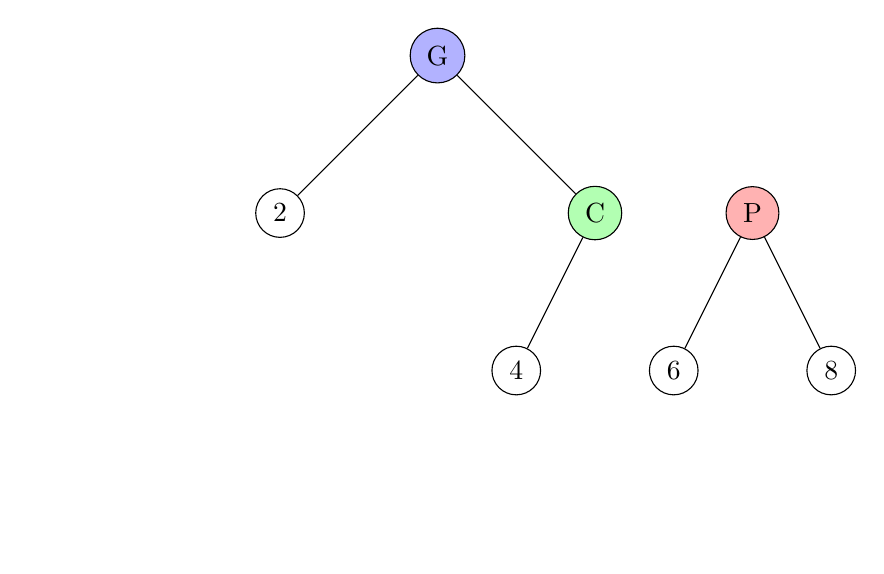
\begin{tikzpicture}
        \begin{scope}{shift={(3,0)}}
            \node[opacity=0] (X) at (-1, 2) { $1$ };
            \node[circle,draw,fill=blue!30] (A) at (4, 8) { G };
            \node[circle,draw] (B) at (2, 6) { 2 };
            \node[circle,draw,fill=red!30] (C) at (8, 6) { P };
            \node[circle,draw,fill=green!30] (D) at (6, 6) { C };
            \node[circle,draw] (E) at (9, 4) { 8 };
            \node[circle,draw] (F) at (5, 4) { 4 };
            \node[circle,draw] (G) at (7, 4) { 6 };

            \draw (A) -- (B);
            \draw (A) -- (D);
            \draw (C) -- (E);
            \draw (D) -- (F);
            \draw (C) -- (G);
        \end{scope}
    \end{tikzpicture}

\end{frame}

\begin{frame}
\frametitle{Exemplo de rotação à direita}

    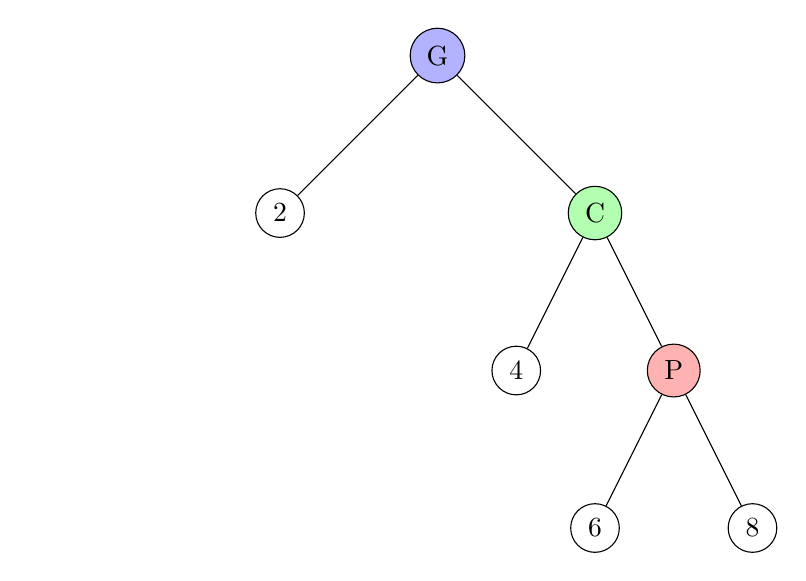
\begin{tikzpicture}
        \begin{scope}{shift={(3,0)}}
            \node[opacity=0] (X) at (-1, 2) { $1$ };
            \node[circle,draw,fill=blue!30] (A) at (4, 8) { G };
            \node[circle,draw] (B) at (2, 6) { 2 };
            \node[circle,draw,fill=red!30] (C) at (7, 4) { P };
            \node[circle,draw,fill=green!30] (D) at (6, 6) { C };
            \node[circle,draw] (E) at (8, 2) { 8 };
            \node[circle,draw] (F) at (5, 4) { 4 };
            \node[circle,draw] (G) at (6, 2) { 6 };

            \draw (A) -- (B);
            \draw (A) -- (D);
            \draw (C) -- (E);
            \draw (C) -- (D);
            \draw (D) -- (F);
            \draw (C) -- (G);
        \end{scope}
    \end{tikzpicture}

\end{frame}

\begin{frame}{Algoritmo DSW}

	\begin{itemize}
		\item O algoritmo DSW é composto por duas etapas

        \item A primeira delas consiste em {transformar} a árvore em uma lista encadeada 
            denominada {espinha dorsal} (\textit{backbone})

        \item Em seguida o algoritmo transforma esta espinha dorsal numa árvore completa

		\item Estas duas etapas são realizada através do uso das {rotações} descritas anteriormente

        \item Cada rotação preserva a estrutura da árvore binária de busca, mudando contudo sua
            forma
	\end{itemize}

\end{frame}

\begin{frame}[fragile]{Geração da espinha dorsal}

    \begin{itemize}
        \item A espinha dorsal é gerada através de sucessivas aplicações de rotações à direita

        \item Inicialmente se inicializa o filho \code{c}{C} na raiz da árvore 
            (naturalmente, o pai \code{c}{P} e o avô \code{c}{G} são inicialmente nulos)

        \item Se \code{c}{C} tem um filho à esquerda, este passa a ser o filho e \code{c}{C} passa
            a ser o pai, e em seguida é aplicada uma rotação à direita

        \item \textit{Corner case}: se, no início do passo anterior, \code{c}{C} era a raiz da
            árvore, a raiz deve apontar para o filho à esquerda antes da rotação

        \item Se \code{c}{C} não tem filhos à esquerda, 
            \code{c}{G} passa a armazenar o valor de \code{c}{C} e \code{c}{C}
            passa a apontar para o seu filho à direita

        \item Quando \code{c}{C} apontar para nulo, a árvore estará completamente degenerada,
            formando a espinha dorsal
    \end{itemize}

\end{frame}

\begin{frame}
\frametitle{Exemplo de árvore desbalanceada}

    \begin{tikzpicture}
        \begin{scope}{shift={(3,0)}}
            \node[opacity=0] (X) at (1, 2) { $1$ };
            \node[circle,draw] (A) at (4, 8) { 20 };
            \node[circle,draw] (B) at (2, 7) { 10 };
            \node[circle,draw] (C) at (7, 6) { 48 };
            \node[circle,draw] (D) at (6, 7) { 30 };
            \node[circle,draw] (E) at (8, 5) { 55 };
            \node[circle,draw] (F) at (5, 6) { 22 };
            \node[circle,draw] (G) at (6, 5) { 39 };

            \draw (A) -- (B);
            \draw (A) -- (D);
            \draw (C) -- (E);
            \draw (C) -- (D);
            \draw (D) -- (F);
            \draw (C) -- (G);
        \end{scope}
    \end{tikzpicture}

\end{frame}

\begin{frame}
\frametitle{Exemplo de geração do backbone}

    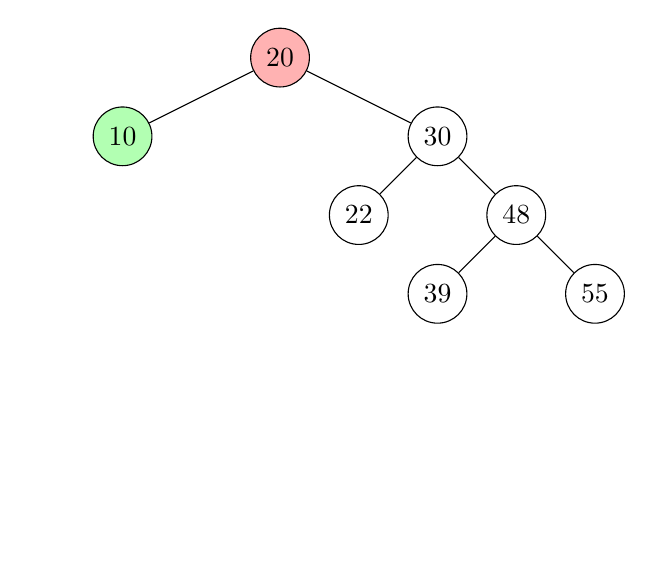
\begin{tikzpicture}
        \begin{scope}{shift={(3,0)}}
            \node[opacity=0] (X) at (1, 2) { $1$ };
            \node[circle,draw,fill=red!30] (A) at (4, 8) { 20 };
            \node[circle,draw,fill=green!30] (B) at (2, 7) { 10 };
            \node[circle,draw] (C) at (7, 6) { 48 };
            \node[circle,draw] (D) at (6, 7) { 30 };
            \node[circle,draw] (E) at (8, 5) { 55 };
            \node[circle,draw] (F) at (5, 6) { 22 };
            \node[circle,draw] (G) at (6, 5) { 39 };

            \draw (A) -- (B);
            \draw (A) -- (D);
            \draw (C) -- (E);
            \draw (C) -- (D);
            \draw (D) -- (F);
            \draw (C) -- (G);
        \end{scope}
    \end{tikzpicture}

\end{frame}

\begin{frame}
\frametitle{Exemplo de geração do backbone}

    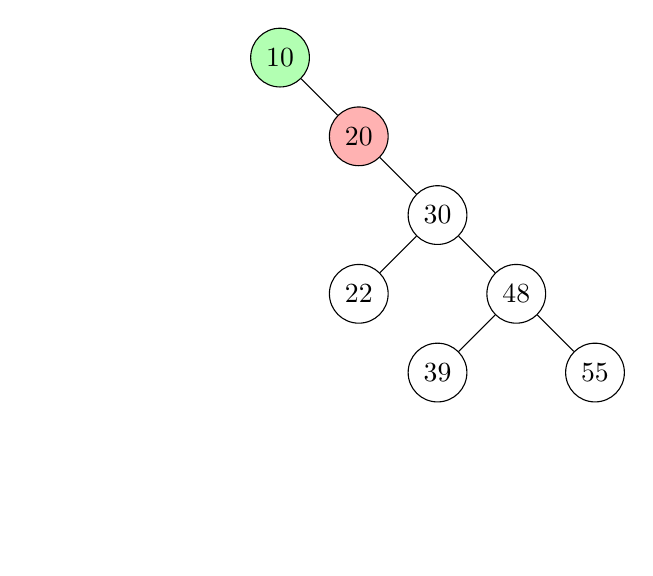
\begin{tikzpicture}
        \begin{scope}{shift={(3,0)}}
            \node[opacity=0] (X) at (1, 2) { $1$ };
            \node[circle,draw,fill=red!30] (A) at (5, 7) { 20 };
            \node[circle,draw,fill=green!30] (B) at (4, 8) { 10 };
            \node[circle,draw] (C) at (7, 5) { 48 };
            \node[circle,draw] (D) at (6, 6) { 30 };
            \node[circle,draw] (E) at (8, 4) { 55 };
            \node[circle,draw] (F) at (5, 5) { 22 };
            \node[circle,draw] (G) at (6, 4) { 39 };

            \draw (A) -- (B);
            \draw (A) -- (D);
            \draw (C) -- (E);
            \draw (C) -- (D);
            \draw (D) -- (F);
            \draw (C) -- (G);
        \end{scope}
    \end{tikzpicture}

\end{frame}

\begin{frame}
\frametitle{Exemplo de geração do backbone}

    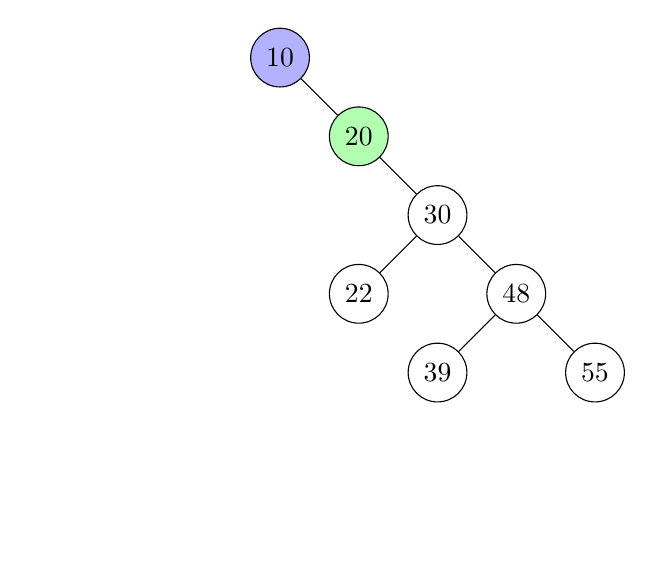
\begin{tikzpicture}
        \begin{scope}{shift={(3,0)}}
            \node[opacity=0] (X) at (1, 2) { $1$ };
            \node[circle,draw,fill=green!30] (A) at (5, 7) { 20 };
            \node[circle,draw,fill=blue!30] (B) at (4, 8) { 10 };
            \node[circle,draw] (C) at (7, 5) { 48 };
            \node[circle,draw] (D) at (6, 6) { 30 };
            \node[circle,draw] (E) at (8, 4) { 55 };
            \node[circle,draw] (F) at (5, 5) { 22 };
            \node[circle,draw] (G) at (6, 4) { 39 };

            \draw (A) -- (B);
            \draw (A) -- (D);
            \draw (C) -- (E);
            \draw (C) -- (D);
            \draw (D) -- (F);
            \draw (C) -- (G);
        \end{scope}
    \end{tikzpicture}

\end{frame}

\begin{frame}
\frametitle{Exemplo de geração do backbone}

    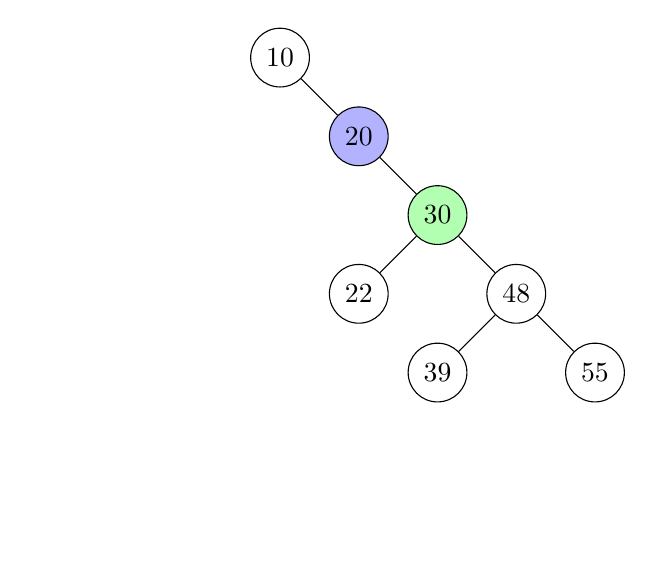
\begin{tikzpicture}
        \begin{scope}{shift={(3,0)}}
            \node[opacity=0] (X) at (1, 2) { $1$ };
            \node[circle,draw,fill=blue!30] (A) at (5, 7) { 20 };
            \node[circle,draw] (B) at (4, 8) { 10 };
            \node[circle,draw] (C) at (7, 5) { 48 };
            \node[circle,draw,fill=green!30] (D) at (6, 6) { 30 };
            \node[circle,draw] (E) at (8, 4) { 55 };
            \node[circle,draw] (F) at (5, 5) { 22 };
            \node[circle,draw] (G) at (6, 4) { 39 };

            \draw (A) -- (B);
            \draw (A) -- (D);
            \draw (C) -- (E);
            \draw (C) -- (D);
            \draw (D) -- (F);
            \draw (C) -- (G);
        \end{scope}
    \end{tikzpicture}

\end{frame}

\begin{frame}
\frametitle{Exemplo de geração do backbone}

    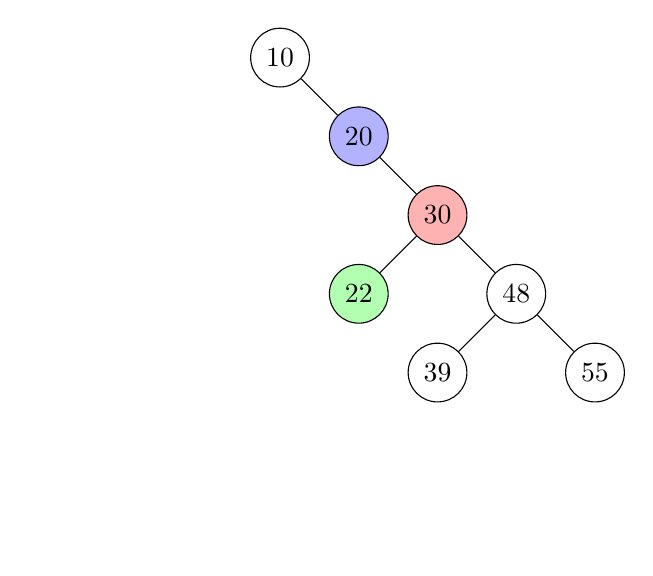
\begin{tikzpicture}
        \begin{scope}{shift={(3,0)}}
            \node[opacity=0] (X) at (1, 2) { $1$ };
            \node[circle,draw,fill=blue!30] (A) at (5, 7) { 20 };
            \node[circle,draw] (B) at (4, 8) { 10 };
            \node[circle,draw] (C) at (7, 5) { 48 };
            \node[circle,draw,fill=red!30] (D) at (6, 6) { 30 };
            \node[circle,draw] (E) at (8, 4) { 55 };
            \node[circle,draw,fill=green!30] (F) at (5, 5) { 22 };
            \node[circle,draw] (G) at (6, 4) { 39 };

            \draw (A) -- (B);
            \draw (A) -- (D);
            \draw (C) -- (E);
            \draw (C) -- (D);
            \draw (D) -- (F);
            \draw (C) -- (G);
        \end{scope}
    \end{tikzpicture}

\end{frame}

\begin{frame}
\frametitle{Exemplo de geração do backbone}

    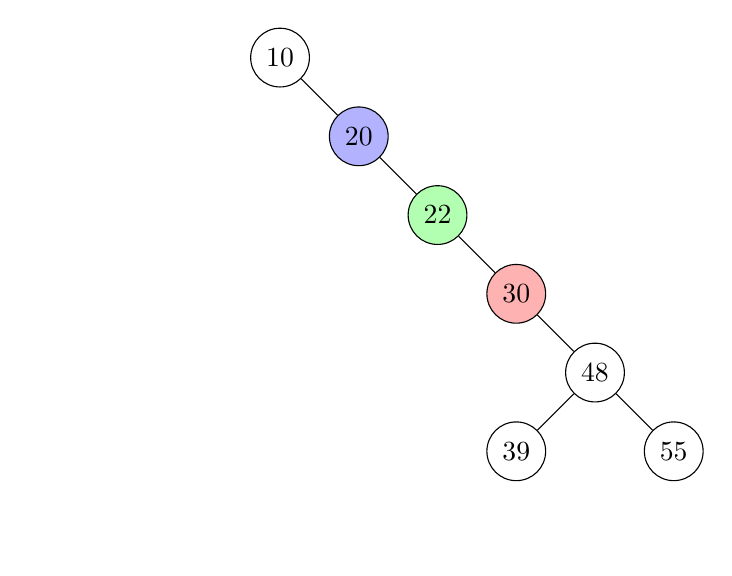
\begin{tikzpicture}
        \begin{scope}{shift={(3,0)}}
            \node[opacity=0] (X) at (1, 2) { $1$ };
            \node[circle,draw,fill=blue!30] (A) at (5, 7) { 20 };
            \node[circle,draw] (B) at (4, 8) { 10 };
            \node[circle,draw] (C) at (8, 4) { 48 };
            \node[circle,draw,fill=red!30] (D) at (7, 5) { 30 };
            \node[circle,draw] (E) at (9, 3) { 55 };
            \node[circle,draw,fill=green!30] (F) at (6, 6) { 22 };
            \node[circle,draw] (G) at (7, 3) { 39 };

            \draw (A) -- (B);
            \draw (A) -- (F);
            \draw (C) -- (E);
            \draw (C) -- (D);
            \draw (D) -- (F);
            \draw (C) -- (G);
        \end{scope}
    \end{tikzpicture}

\end{frame}

\begin{frame}
\frametitle{Exemplo de geração do backbone}

    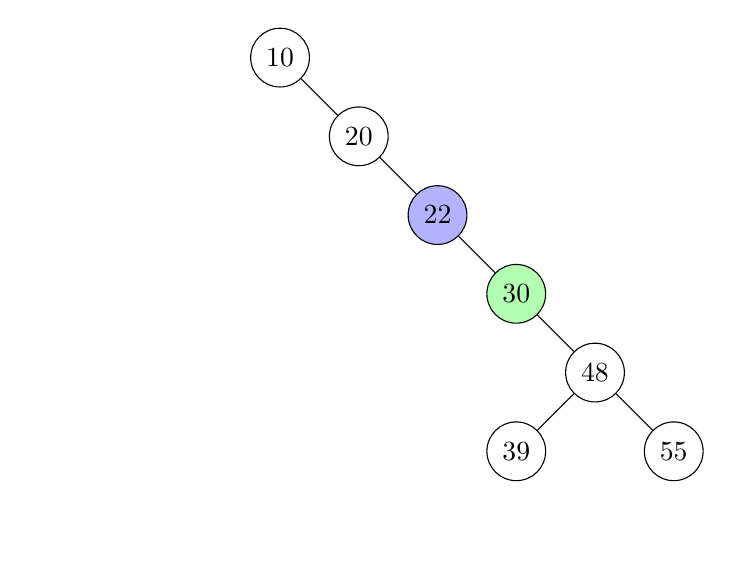
\begin{tikzpicture}
        \begin{scope}{shift={(3,0)}}
            \node[opacity=0] (X) at (1, 2) { $1$ };
            \node[circle,draw] (A) at (5, 7) { 20 };
            \node[circle,draw] (B) at (4, 8) { 10 };
            \node[circle,draw] (C) at (8, 4) { 48 };
            \node[circle,draw,fill=green!30] (D) at (7, 5) { 30 };
            \node[circle,draw] (E) at (9, 3) { 55 };
            \node[circle,draw,fill=blue!30] (F) at (6, 6) { 22 };
            \node[circle,draw] (G) at (7, 3) { 39 };

            \draw (A) -- (B);
            \draw (A) -- (F);
            \draw (C) -- (E);
            \draw (C) -- (D);
            \draw (D) -- (F);
            \draw (C) -- (G);
        \end{scope}
    \end{tikzpicture}

\end{frame}

\begin{frame}
\frametitle{Exemplo de geração do backbone}

    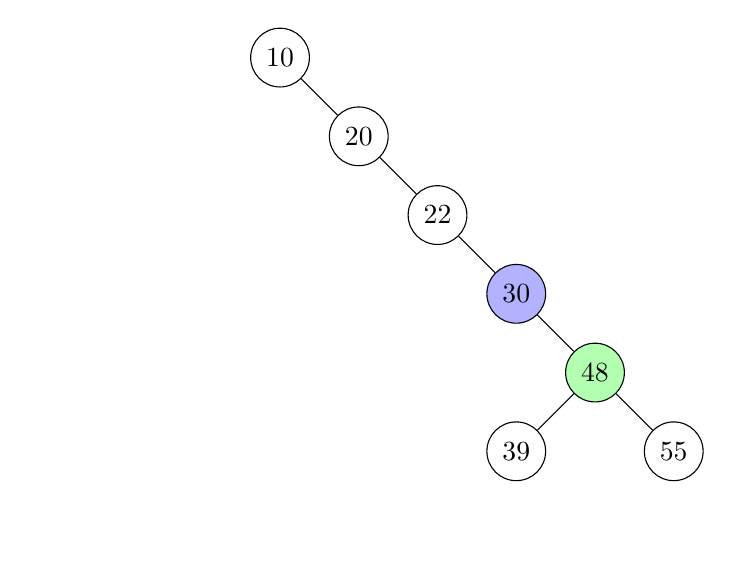
\begin{tikzpicture}
        \begin{scope}{shift={(3,0)}}
            \node[opacity=0] (X) at (1, 2) { $1$ };
            \node[circle,draw] (A) at (5, 7) { 20 };
            \node[circle,draw] (B) at (4, 8) { 10 };
            \node[circle,draw,fill=green!30] (C) at (8, 4) { 48 };
            \node[circle,draw,fill=blue!30] (D) at (7, 5) { 30 };
            \node[circle,draw] (E) at (9, 3) { 55 };
            \node[circle,draw] (F) at (6, 6) { 22 };
            \node[circle,draw] (G) at (7, 3) { 39 };

            \draw (A) -- (B);
            \draw (A) -- (F);
            \draw (C) -- (E);
            \draw (C) -- (D);
            \draw (D) -- (F);
            \draw (C) -- (G);
        \end{scope}
    \end{tikzpicture}

\end{frame}

\begin{frame}
\frametitle{Exemplo de geração do backbone}

    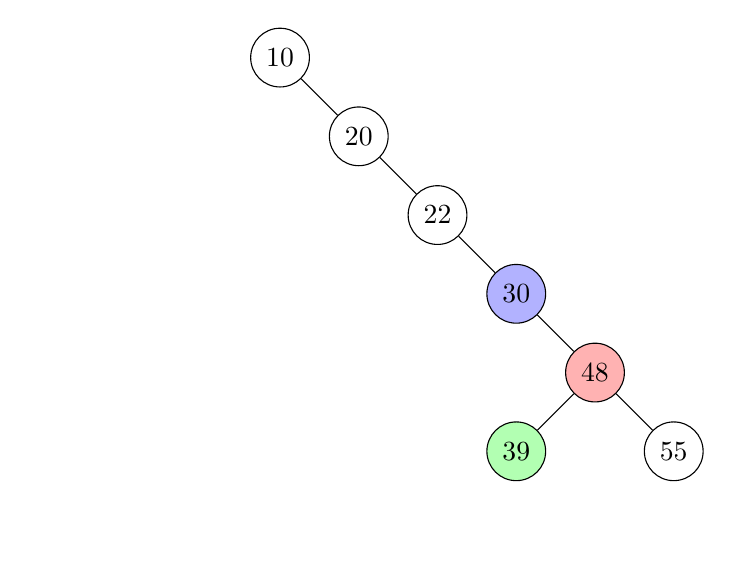
\begin{tikzpicture}
        \begin{scope}{shift={(3,0)}}
            \node[opacity=0] (X) at (1, 2) { $1$ };
            \node[circle,draw] (A) at (5, 7) { 20 };
            \node[circle,draw] (B) at (4, 8) { 10 };
            \node[circle,draw,fill=red!30] (C) at (8, 4) { 48 };
            \node[circle,draw,fill=blue!30] (D) at (7, 5) { 30 };
            \node[circle,draw] (E) at (9, 3) { 55 };
            \node[circle,draw] (F) at (6, 6) { 22 };
            \node[circle,draw,fill=green!30] (G) at (7, 3) { 39 };

            \draw (A) -- (B);
            \draw (A) -- (F);
            \draw (C) -- (E);
            \draw (C) -- (D);
            \draw (D) -- (F);
            \draw (C) -- (G);
        \end{scope}
    \end{tikzpicture}

\end{frame}

\begin{frame}
\frametitle{Exemplo de geração do backbone}

    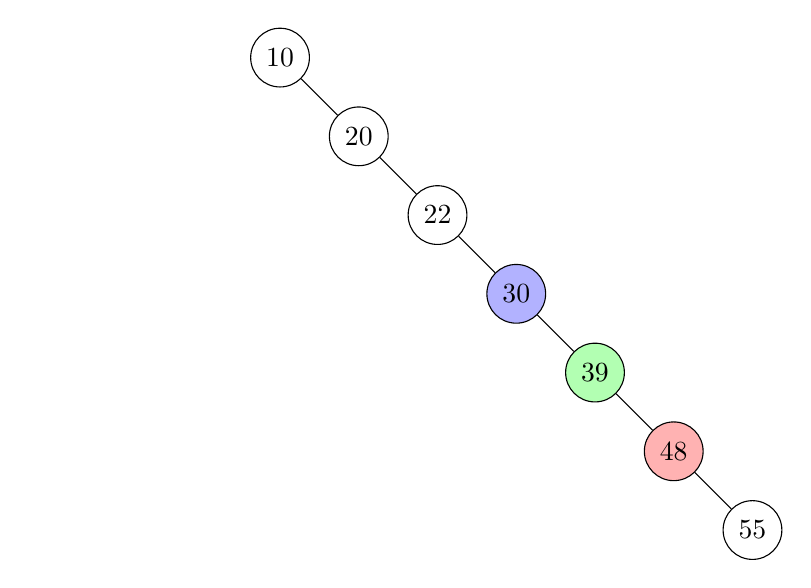
\begin{tikzpicture}
        \begin{scope}{shift={(3,0)}}
            \node[opacity=0] (X) at (1, 2) { $1$ };
            \node[circle,draw] (A) at (5, 7) { 20 };
            \node[circle,draw] (B) at (4, 8) { 10 };
            \node[circle,draw,fill=red!30] (C) at (9, 3) { 48 };
            \node[circle,draw,fill=blue!30] (D) at (7, 5) { 30 };
            \node[circle,draw] (E) at (10, 2) { 55 };
            \node[circle,draw] (F) at (6, 6) { 22 };
            \node[circle,draw,fill=green!30] (G) at (8, 4) { 39 };

            \draw (A) -- (B);
            \draw (A) -- (F);
            \draw (C) -- (E);
            \draw (D) -- (G);
            \draw (D) -- (F);
            \draw (C) -- (G);
        \end{scope}
    \end{tikzpicture}

\end{frame}

\begin{frame}
\frametitle{Exemplo de geração do backbone}

    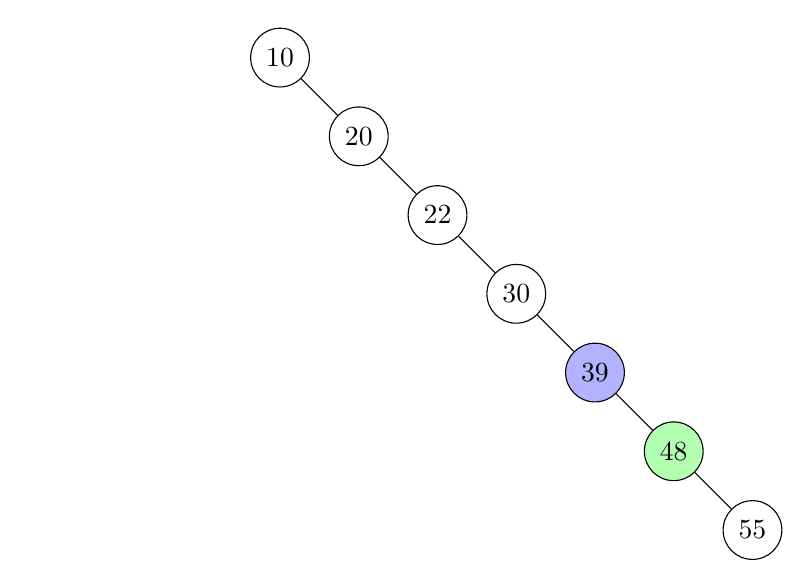
\begin{tikzpicture}
        \begin{scope}{shift={(3,0)}}
            \node[opacity=0] (X) at (1, 2) { $1$ };
            \node[circle,draw] (A) at (5, 7) { 20 };
            \node[circle,draw] (B) at (4, 8) { 10 };
            \node[circle,draw,fill=green!30] (C) at (9, 3) { 48 };
            \node[circle,draw] (D) at (7, 5) { 30 };
            \node[circle,draw] (E) at (10, 2) { 55 };
            \node[circle,draw] (F) at (6, 6) { 22 };
            \node[circle,draw,fill=blue!30] (G) at (8, 4) { 39 };

            \draw (A) -- (B);
            \draw (A) -- (F);
            \draw (C) -- (E);
            \draw (D) -- (G);
            \draw (D) -- (F);
            \draw (C) -- (G);
        \end{scope}
    \end{tikzpicture}

\end{frame}

\begin{frame}
\frametitle{Exemplo de geração do backbone}

    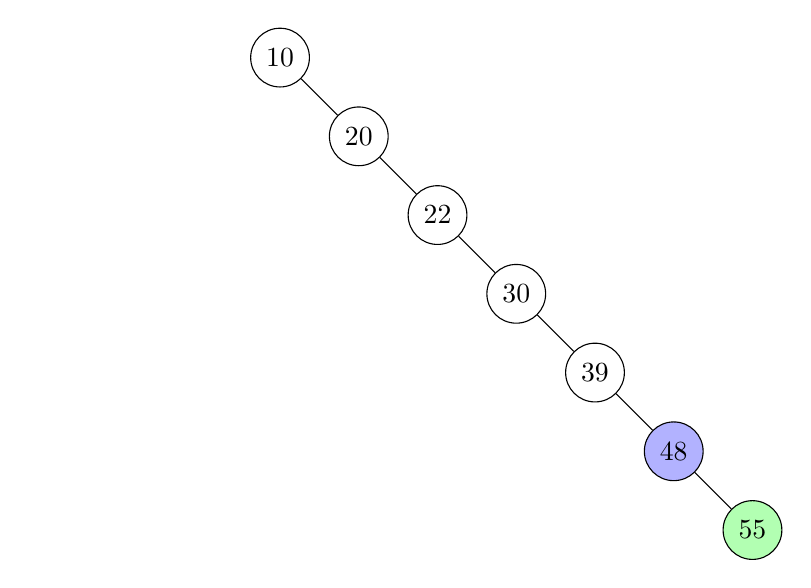
\begin{tikzpicture}
        \begin{scope}{shift={(3,0)}}
            \node[opacity=0] (X) at (1, 2) { $1$ };
            \node[circle,draw] (A) at (5, 7) { 20 };
            \node[circle,draw] (B) at (4, 8) { 10 };
            \node[circle,draw,fill=blue!30] (C) at (9, 3) { 48 };
            \node[circle,draw] (D) at (7, 5) { 30 };
            \node[circle,draw,fill=green!30] (E) at (10, 2) { 55 };
            \node[circle,draw] (F) at (6, 6) { 22 };
            \node[circle,draw] (G) at (8, 4) { 39 };

            \draw (A) -- (B);
            \draw (A) -- (F);
            \draw (C) -- (E);
            \draw (D) -- (G);
            \draw (D) -- (F);
            \draw (C) -- (G);
        \end{scope}
    \end{tikzpicture}

\end{frame}

\begin{frame}[fragile]{Implementação da geração da espinha dorsal}
    \inputsnippet{cpp}{1}{13}{backbone.cpp}
\end{frame}

\begin{frame}[fragile]{Implementação da geração da espinha dorsal}
    \inputsnippet{cpp}{14}{34}{backbone.cpp}
\end{frame}

\begin{frame}[fragile]{Reorganização da espinha dorsal em uma árvore perfeitamente balanceada}

    \begin{itemize}
        \item Com o objetivo de gerar uma árvore perfeitamente balanceada a partir da espinha
            dorsal é definida uma função de transformação

        \item Esta função realiza uma série de rotações à esquerda

        \item Antes de cada rotação, os ponteiros \code{c}{G, P, C} são atualizados, movendo-se
            para a esquerda, dois passos por vez

        \item Os dois casos especiais envolvem a raiz

        \item Se o pai aponta para nulo, o filho será a raiz da árvore

        \item Se o pai for a raiz, a raiz passará a ser igual ao filho

        \item O número de rotações a serem feitas está relacionado com o logaritmo de $N$ na 
            base 2, onde $N$ é o número de nós da árvore
    \end{itemize}

\end{frame}


\begin{frame}[fragile]{Implementação do algoritmo DSW}
    \inputsnippet{cpp}{1}{21}{dsw.cpp}
\end{frame}

\begin{frame}[fragile]{Implementação do algoritmo DSW}
    \inputsnippet{cpp}{22}{42}{dsw.cpp}
\end{frame}

\begin{frame}[fragile]{Implementação do algoritmo DSW}
    \inputsnippet{cpp}{43}{63}{dsw.cpp}
\end{frame}

\begin{frame}
\frametitle{Algoritmo DSW: transformação da espinha dorsal}

    \begin{tikzpicture}
        \begin{scope}{shift={(3,0)}}
            \node[opacity=0] (X) at (1, 2) { $1$ };
            \node[circle,draw] (A) at (5, 7) { 20 };
            \node[circle,draw] (B) at (4, 8) { 10 };
            \node[circle,draw] (C) at (9, 3) { 48 };
            \node[circle,draw] (D) at (7, 5) { 30 };
            \node[circle,draw] (E) at (10, 2) { 55 };
            \node[circle,draw] (F) at (6, 6) { 22 };
            \node[circle,draw] (G) at (8, 4) { 39 };
            \node[circle,draw] (H) at (11, 1) { 67 };

            \draw (A) -- (B);
            \draw (A) -- (F);
            \draw (C) -- (E);
            \draw (D) -- (G);
            \draw (D) -- (F);
            \draw (C) -- (G);
            \draw (E) -- (H);

            \node[anchor=west] at (7, 8) { N = 8, M = 7 };
        \end{scope}
    \end{tikzpicture}

\end{frame}

\begin{frame}
\frametitle{Algoritmo DSW: transformação da espinha dorsal}

    \begin{tikzpicture}
        \begin{scope}{shift={(3,0)}}
            \node[opacity=0] (X) at (1, 2) { $1$ };
            \node[circle,draw] (A) at (5, 7) { 20 };
            \node[circle,draw] (B) at (4, 8) { 10 };
            \node[circle,draw] (C) at (9, 3) { 48 };
            \node[circle,draw] (D) at (7, 5) { 30 };
            \node[circle,draw] (E) at (10, 2) { 55 };
            \node[circle,draw] (F) at (6, 6) { 22 };
            \node[circle,draw] (G) at (8, 4) { 39 };
            \node[circle,draw] (H) at (11, 1) { 67 };

            \draw (A) -- (B);
            \draw (A) -- (F);
            \draw (C) -- (E);
            \draw (D) -- (G);
            \draw (D) -- (F);
            \draw (C) -- (G);
            \draw (E) -- (H);

            \node[anchor=west] at (7, 8) { N = 8, M = 7, \texttt{transform(1)}};
        \end{scope}
    \end{tikzpicture}

\end{frame}

\begin{frame}
\frametitle{Algoritmo DSW: transformação da espinha dorsal}

    \begin{tikzpicture}
        \begin{scope}{shift={(3,0)}}
            \node[opacity=0] (X) at (1, 2) { $1$ };
            \node[circle,draw] (A) at (5, 7) { 20 };
            \node[circle,draw,fill=green!30] (B) at (4, 8) { 10 };
            \node[circle,draw] (C) at (9, 3) { 48 };
            \node[circle,draw] (D) at (7, 5) { 30 };
            \node[circle,draw] (E) at (10, 2) { 55 };
            \node[circle,draw] (F) at (6, 6) { 22 };
            \node[circle,draw] (G) at (8, 4) { 39 };
            \node[circle,draw] (H) at (11, 1) { 67 };

            \draw (A) -- (B);
            \draw (A) -- (F);
            \draw (C) -- (E);
            \draw (D) -- (G);
            \draw (D) -- (F);
            \draw (C) -- (G);
            \draw (E) -- (H);

            \node[anchor=west] at (7, 8) { N = 8, M = 7, \texttt{transform(1)}};
        \end{scope}
    \end{tikzpicture}

\end{frame}

\begin{frame}
\frametitle{Algoritmo DSW: transformação da espinha dorsal}

    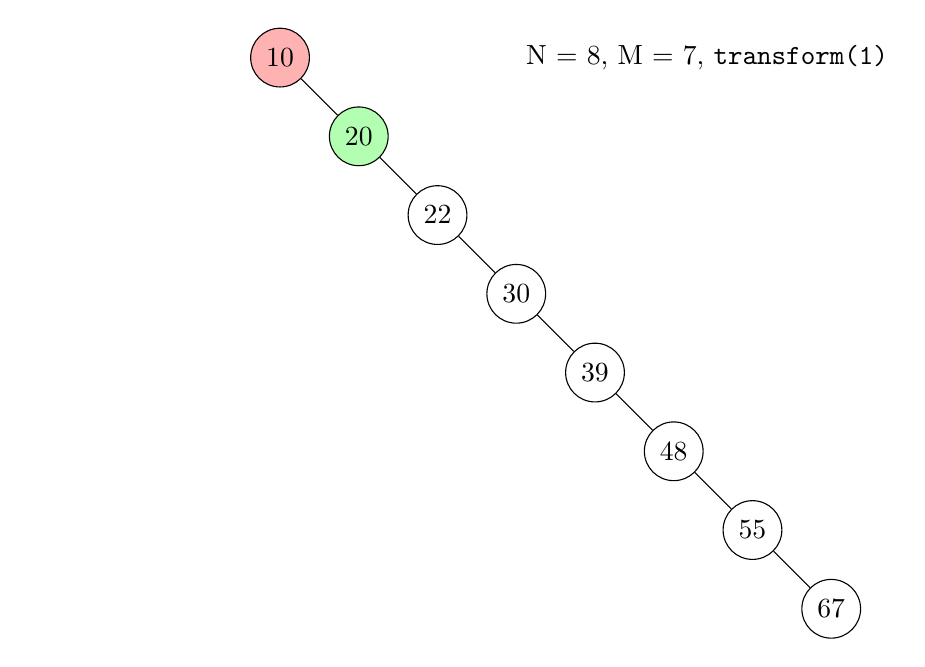
\begin{tikzpicture}
        \begin{scope}{shift={(3,0)}}
            \node[opacity=0] (X) at (1, 2) { $1$ };
            \node[circle,draw,fill=green!30] (A) at (5, 7) { 20 };
            \node[circle,draw,fill=red!30] (B) at (4, 8) { 10 };
            \node[circle,draw] (C) at (9, 3) { 48 };
            \node[circle,draw] (D) at (7, 5) { 30 };
            \node[circle,draw] (E) at (10, 2) { 55 };
            \node[circle,draw] (F) at (6, 6) { 22 };
            \node[circle,draw] (G) at (8, 4) { 39 };
            \node[circle,draw] (H) at (11, 1) { 67 };

            \draw (A) -- (B);
            \draw (A) -- (F);
            \draw (C) -- (E);
            \draw (D) -- (G);
            \draw (D) -- (F);
            \draw (C) -- (G);
            \draw (E) -- (H);

            \node[anchor=west] at (7, 8) { N = 8, M = 7, \texttt{transform(1)}};
        \end{scope}
    \end{tikzpicture}

\end{frame}

\begin{frame}
\frametitle{Algoritmo DSW: transformação da espinha dorsal}

    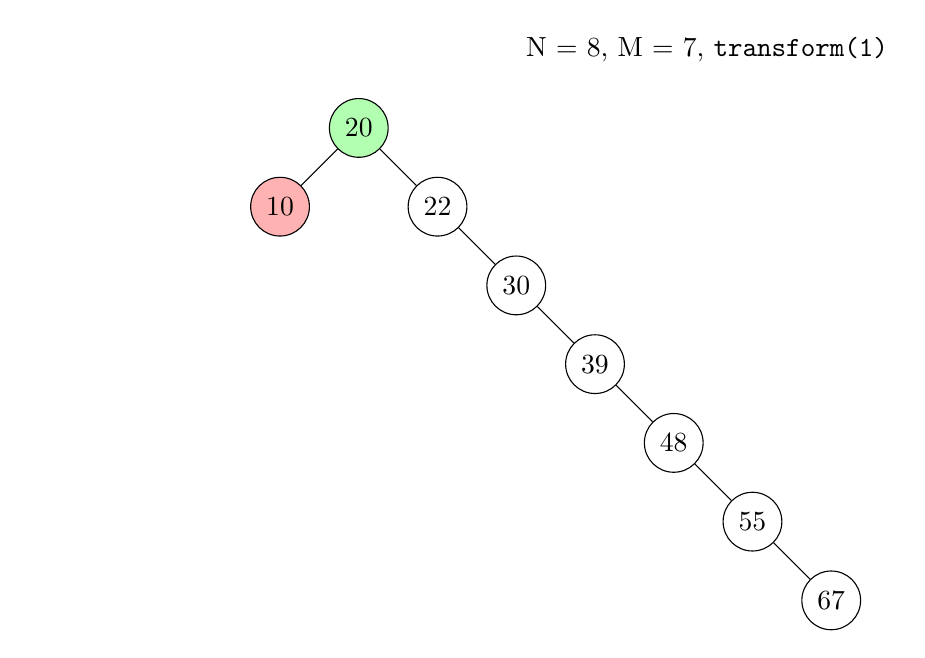
\begin{tikzpicture}
        \begin{scope}{shift={(3,0)}}
            \node[opacity=0] (X) at (1, 2) { $1$ };
            \node[circle,draw,fill=green!30] (A) at (5, 7) { 20 };
            \node[circle,draw,fill=red!30] (B) at (4, 6) { 10 };
            \node[circle,draw] (C) at (9, 3) { 48 };
            \node[circle,draw] (D) at (7, 5) { 30 };
            \node[circle,draw] (E) at (10, 2) { 55 };
            \node[circle,draw] (F) at (6, 6) { 22 };
            \node[circle,draw] (G) at (8, 4) { 39 };
            \node[circle,draw] (H) at (11, 1) { 67 };

            \draw (A) -- (B);
            \draw (A) -- (F);
            \draw (C) -- (E);
            \draw (D) -- (G);
            \draw (D) -- (F);
            \draw (C) -- (G);
            \draw (E) -- (H);

            \node[anchor=west] at (7, 8) { N = 8, M = 7, \texttt{transform(1)}};
        \end{scope}
    \end{tikzpicture}

\end{frame}

\begin{frame}
\frametitle{Algoritmo DSW: transformação da espinha dorsal}

    \begin{tikzpicture}
        \begin{scope}{shift={(3,0)}}
            \node[opacity=0] (X) at (1, 2) { $1$ };
            \node[circle,draw] (A) at (5, 7) { 20 };
            \node[circle,draw] (B) at (4, 6) { 10 };
            \node[circle,draw] (C) at (9, 3) { 48 };
            \node[circle,draw] (D) at (7, 5) { 30 };
            \node[circle,draw] (E) at (10, 2) { 55 };
            \node[circle,draw] (F) at (6, 6) { 22 };
            \node[circle,draw] (G) at (8, 4) { 39 };
            \node[circle,draw] (H) at (11, 1) { 67 };

            \draw (A) -- (B);
            \draw (A) -- (F);
            \draw (C) -- (E);
            \draw (D) -- (G);
            \draw (D) -- (F);
            \draw (C) -- (G);
            \draw (E) -- (H);

            \node[anchor=west] at (7, 8) { N = 8, \textcolor{blue}{M = 3}, \texttt{transform(3)} };
        \end{scope}
    \end{tikzpicture}

\end{frame}

\begin{frame}
\frametitle{Algoritmo DSW: transformação da espinha dorsal}

    \begin{tikzpicture}
        \begin{scope}{shift={(3,0)}}
            \node[opacity=0] (X) at (1, 2) { $1$ };
            \node[circle,draw,fill=green!30] (A) at (5, 7) { 20 };
            \node[circle,draw] (B) at (4, 6) { 10 };
            \node[circle,draw] (C) at (9, 3) { 48 };
            \node[circle,draw] (D) at (7, 5) { 30 };
            \node[circle,draw] (E) at (10, 2) { 55 };
            \node[circle,draw] (F) at (6, 6) { 22 };
            \node[circle,draw] (G) at (8, 4) { 39 };
            \node[circle,draw] (H) at (11, 1) { 67 };

            \draw (A) -- (B);
            \draw (A) -- (F);
            \draw (C) -- (E);
            \draw (D) -- (G);
            \draw (D) -- (F);
            \draw (C) -- (G);
            \draw (E) -- (H);

            \node[anchor=west] at (7, 8) { N = 8, M = 3, \texttt{transform(3)} };
        \end{scope}
    \end{tikzpicture}

\end{frame}

\begin{frame}
\frametitle{Algoritmo DSW: transformação da espinha dorsal}

    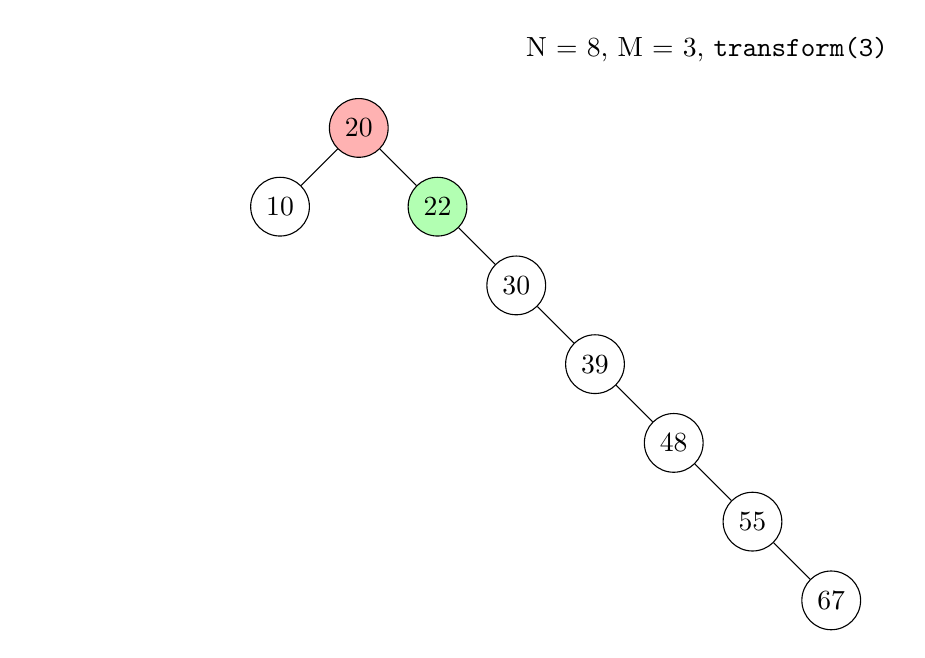
\begin{tikzpicture}
        \begin{scope}{shift={(3,0)}}
            \node[opacity=0] (X) at (1, 2) { $1$ };
            \node[circle,draw,fill=red!30] (A) at (5, 7) { 20 };
            \node[circle,draw] (B) at (4, 6) { 10 };
            \node[circle,draw] (C) at (9, 3) { 48 };
            \node[circle,draw] (D) at (7, 5) { 30 };
            \node[circle,draw] (E) at (10, 2) { 55 };
            \node[circle,draw,fill=green!30] (F) at (6, 6) { 22 };
            \node[circle,draw] (G) at (8, 4) { 39 };
            \node[circle,draw] (H) at (11, 1) { 67 };

            \draw (A) -- (B);
            \draw (A) -- (F);
            \draw (C) -- (E);
            \draw (D) -- (G);
            \draw (D) -- (F);
            \draw (C) -- (G);
            \draw (E) -- (H);

            \node[anchor=west] at (7, 8) { N = 8, M = 3, \texttt{transform(3)} };
        \end{scope}
    \end{tikzpicture}

\end{frame}

\begin{frame}
\frametitle{Algoritmo DSW: transformação da espinha dorsal}

    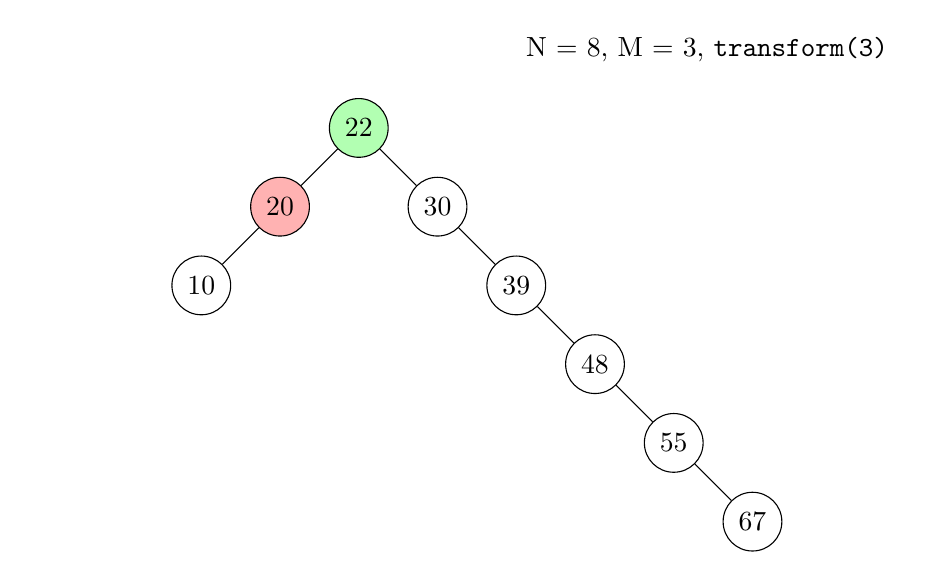
\begin{tikzpicture}
        \begin{scope}{shift={(3,0)}}
            \node[opacity=0] (X) at (1, 2) { $1$ };
            \node[circle,draw,fill=red!30] (A) at (4, 6) { 20 };
            \node[circle,draw] (B) at (3, 5) { 10 };
            \node[circle,draw] (C) at (8, 4) { 48 };
            \node[circle,draw] (D) at (6, 6) { 30 };
            \node[circle,draw] (E) at (9, 3) { 55 };
            \node[circle,draw,fill=green!30] (F) at (5, 7) { 22 };
            \node[circle,draw] (G) at (7, 5) { 39 };
            \node[circle,draw] (H) at (10, 2) { 67 };

            \draw (A) -- (B);
            \draw (A) -- (F);
            \draw (C) -- (E);
            \draw (D) -- (G);
            \draw (D) -- (F);
            \draw (C) -- (G);
            \draw (E) -- (H);

            \node[anchor=west] at (7, 8) { N = 8, M = 3, \texttt{transform(3)} };
        \end{scope}
    \end{tikzpicture}

\end{frame}

\begin{frame}
\frametitle{Algoritmo DSW: transformação da espinha dorsal}

    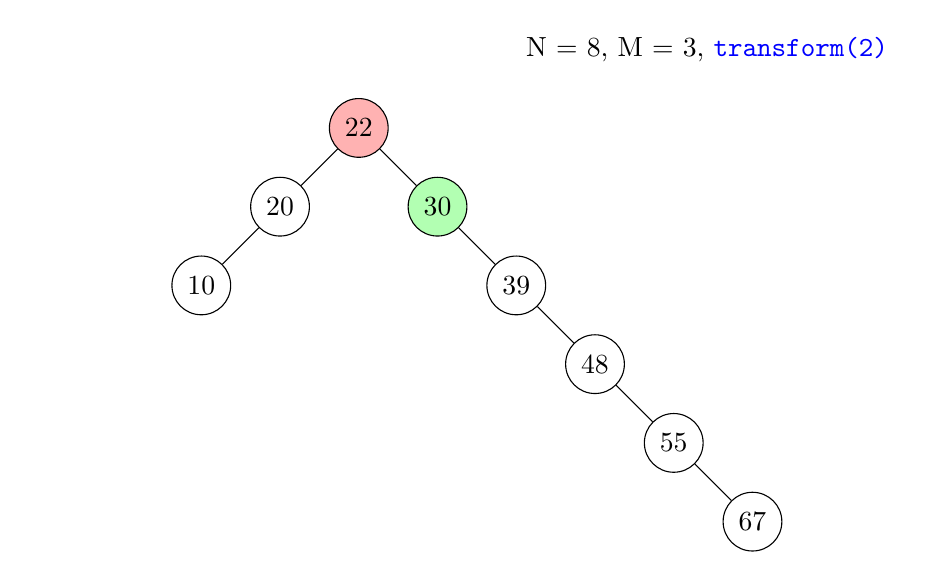
\begin{tikzpicture}
        \begin{scope}{shift={(3,0)}}
            \node[opacity=0] (X) at (1, 2) { $1$ };
            \node[circle,draw] (A) at (4, 6) { 20 };
            \node[circle,draw] (B) at (3, 5) { 10 };
            \node[circle,draw] (C) at (8, 4) { 48 };
            \node[circle,draw,fill=green!30] (D) at (6, 6) { 30 };
            \node[circle,draw] (E) at (9, 3) { 55 };
            \node[circle,draw,fill=red!30] (F) at (5, 7) { 22 };
            \node[circle,draw] (G) at (7, 5) { 39 };
            \node[circle,draw] (H) at (10, 2) { 67 };

            \draw (A) -- (B);
            \draw (A) -- (F);
            \draw (C) -- (E);
            \draw (D) -- (G);
            \draw (D) -- (F);
            \draw (C) -- (G);
            \draw (E) -- (H);

            \node[anchor=west] at (7, 8) { N = 8, M = 3, \textcolor{blue}{\texttt{transform(2)}} };
        \end{scope}
    \end{tikzpicture}

\end{frame}

\begin{frame}
\frametitle{Algoritmo DSW: transformação da espinha dorsal}

    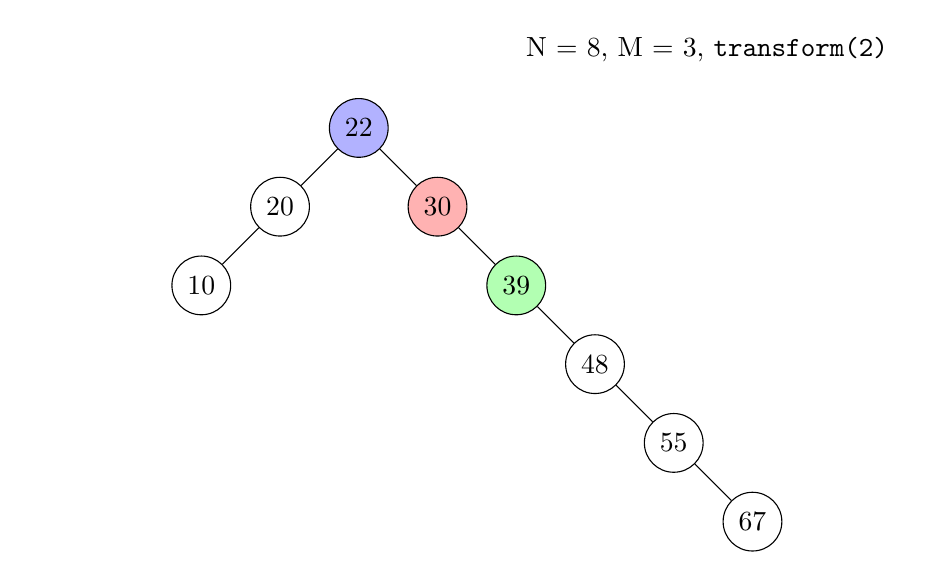
\begin{tikzpicture}
        \begin{scope}{shift={(3,0)}}
            \node[opacity=0] (X) at (1, 2) { $1$ };
            \node[circle,draw] (A) at (4, 6) { 20 };
            \node[circle,draw] (B) at (3, 5) { 10 };
            \node[circle,draw] (C) at (8, 4) { 48 };
            \node[circle,draw,fill=red!30] (D) at (6, 6) { 30 };
            \node[circle,draw] (E) at (9, 3) { 55 };
            \node[circle,draw,fill=blue!30] (F) at (5, 7) { 22 };
            \node[circle,draw,fill=green!30] (G) at (7, 5) { 39 };
            \node[circle,draw] (H) at (10, 2) { 67 };

            \draw (A) -- (B);
            \draw (A) -- (F);
            \draw (C) -- (E);
            \draw (D) -- (G);
            \draw (D) -- (F);
            \draw (C) -- (G);
            \draw (E) -- (H);

            \node[anchor=west] at (7, 8) { N = 8, M = 3, \textcolor{black}{\texttt{transform(2)}} };
        \end{scope}
    \end{tikzpicture}

\end{frame}

\begin{frame}
\frametitle{Algoritmo DSW: transformação da espinha dorsal}

    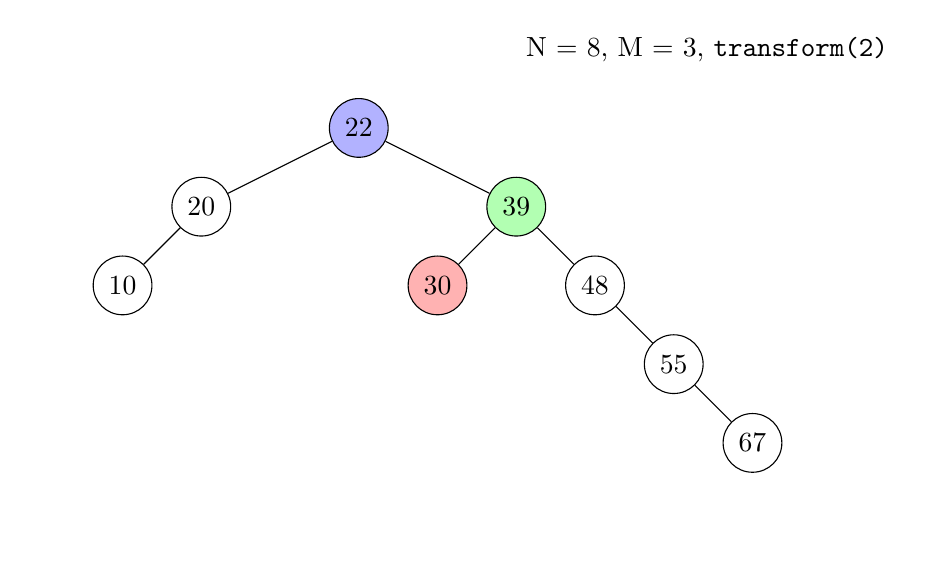
\begin{tikzpicture}
        \begin{scope}{shift={(3,0)}}
            \node[opacity=0] (X) at (1, 2) { $1$ };
            \node[circle,draw] (A) at (3, 6) { 20 };
            \node[circle,draw] (B) at (2, 5) { 10 };
            \node[circle,draw] (C) at (8, 5) { 48 };
            \node[circle,draw,fill=red!30] (D) at (6, 5) { 30 };
            \node[circle,draw] (E) at (9, 4) { 55 };
            \node[circle,draw,fill=blue!30] (F) at (5, 7) { 22 };
            \node[circle,draw,fill=green!30] (G) at (7, 6) { 39 };
            \node[circle,draw] (H) at (10, 3) { 67 };

            \draw (A) -- (B);
            \draw (A) -- (F);
            \draw (C) -- (E);
            \draw (F) -- (G);
            \draw (D) -- (G);
            \draw (C) -- (G);
            \draw (E) -- (H);

            \node[anchor=west] at (7, 8) { N = 8, M = 3, \textcolor{black}{\texttt{transform(2)}} };
        \end{scope}
    \end{tikzpicture}

\end{frame}

\begin{frame}
\frametitle{Algoritmo DSW: transformação da espinha dorsal}

    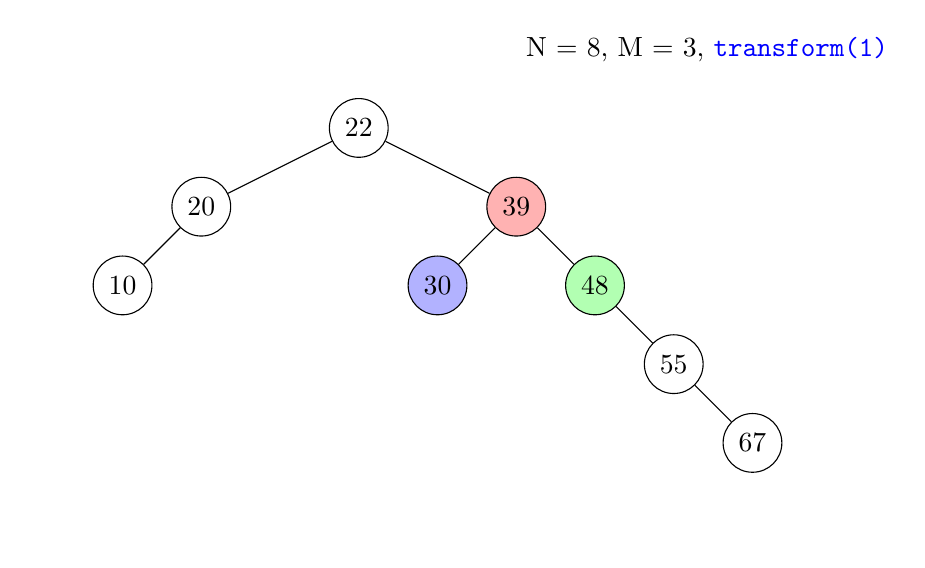
\begin{tikzpicture}
        \begin{scope}{shift={(3,0)}}
            \node[opacity=0] (X) at (1, 2) { $1$ };
            \node[circle,draw] (A) at (3, 6) { 20 };
            \node[circle,draw] (B) at (2, 5) { 10 };
            \node[circle,draw,fill=green!30] (C) at (8, 5) { 48 };
            \node[circle,draw,fill=blue!30] (D) at (6, 5) { 30 };
            \node[circle,draw] (E) at (9, 4) { 55 };
            \node[circle,draw] (F) at (5, 7) { 22 };
            \node[circle,draw,fill=red!30] (G) at (7, 6) { 39 };
            \node[circle,draw] (H) at (10, 3) { 67 };

            \draw (A) -- (B);
            \draw (A) -- (F);
            \draw (C) -- (E);
            \draw (F) -- (G);
            \draw (D) -- (G);
            \draw (C) -- (G);
            \draw (E) -- (H);

            \node[anchor=west] at (7, 8) { N = 8, M = 3, \textcolor{blue}{\texttt{transform(1)}} };
        \end{scope}
    \end{tikzpicture}

\end{frame}

\begin{frame}
\frametitle{Algoritmo DSW: transformação da espinha dorsal}

    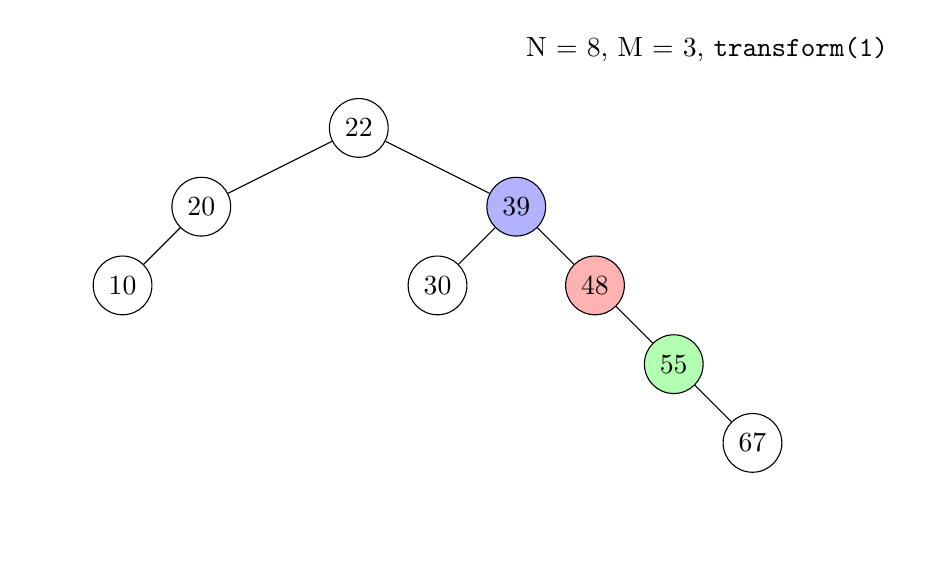
\begin{tikzpicture}
        \begin{scope}{shift={(3,0)}}
            \node[opacity=0] (X) at (1, 2) { $1$ };
            \node[circle,draw] (A) at (3, 6) { 20 };
            \node[circle,draw] (B) at (2, 5) { 10 };
            \node[circle,draw,fill=red!30] (C) at (8, 5) { 48 };
            \node[circle,draw] (D) at (6, 5) { 30 };
            \node[circle,draw,fill=green!30] (E) at (9, 4) { 55 };
            \node[circle,draw] (F) at (5, 7) { 22 };
            \node[circle,draw,fill=blue!30] (G) at (7, 6) { 39 };
            \node[circle,draw] (H) at (10, 3) { 67 };

            \draw (A) -- (B);
            \draw (A) -- (F);
            \draw (C) -- (E);
            \draw (F) -- (G);
            \draw (D) -- (G);
            \draw (C) -- (G);
            \draw (E) -- (H);

            \node[anchor=west] at (7, 8) { N = 8, M = 3, \textcolor{black}{\texttt{transform(1)}} };
        \end{scope}
    \end{tikzpicture}

\end{frame}

\begin{frame}
\frametitle{Algoritmo DSW: transformação da espinha dorsal}

    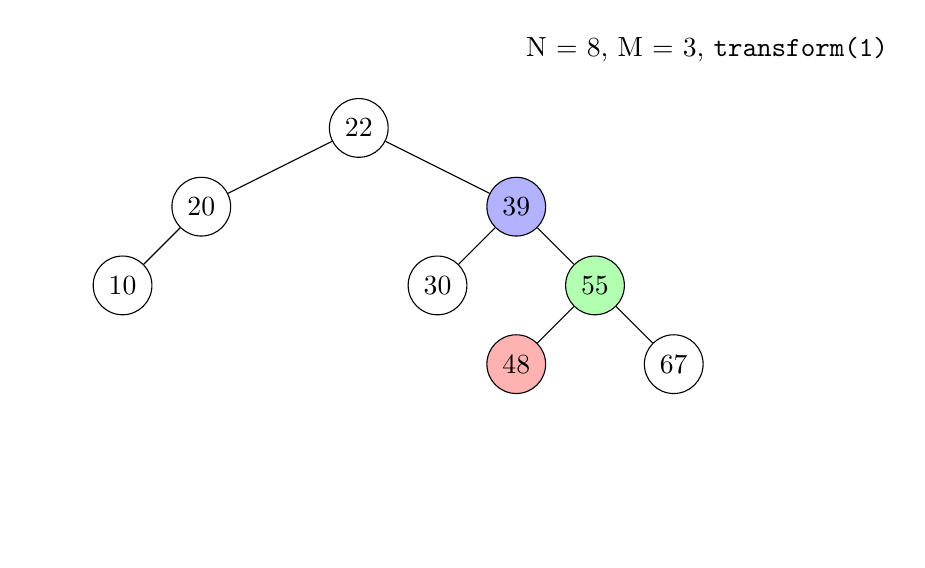
\begin{tikzpicture}
        \begin{scope}{shift={(3,0)}}
            \node[opacity=0] (X) at (1, 2) { $1$ };
            \node[circle,draw] (A) at (3, 6) { 20 };
            \node[circle,draw] (B) at (2, 5) { 10 };
            \node[circle,draw,fill=red!30] (C) at (7, 4) { 48 };
            \node[circle,draw] (D) at (6, 5) { 30 };
            \node[circle,draw,fill=green!30] (E) at (8, 5) { 55 };
            \node[circle,draw] (F) at (5, 7) { 22 };
            \node[circle,draw,fill=blue!30] (G) at (7, 6) { 39 };
            \node[circle,draw] (H) at (9, 4) { 67 };

            \draw (A) -- (B);
            \draw (A) -- (F);
            \draw (C) -- (E);
            \draw (F) -- (G);
            \draw (D) -- (G);
            \draw (E) -- (G);
            \draw (E) -- (H);

            \node[anchor=west] at (7, 8) { N = 8, M = 3, \textcolor{black}{\texttt{transform(1)}} };
        \end{scope}
    \end{tikzpicture}

\end{frame}

\begin{frame}
\frametitle{Algoritmo DSW: transformação da espinha dorsal}

    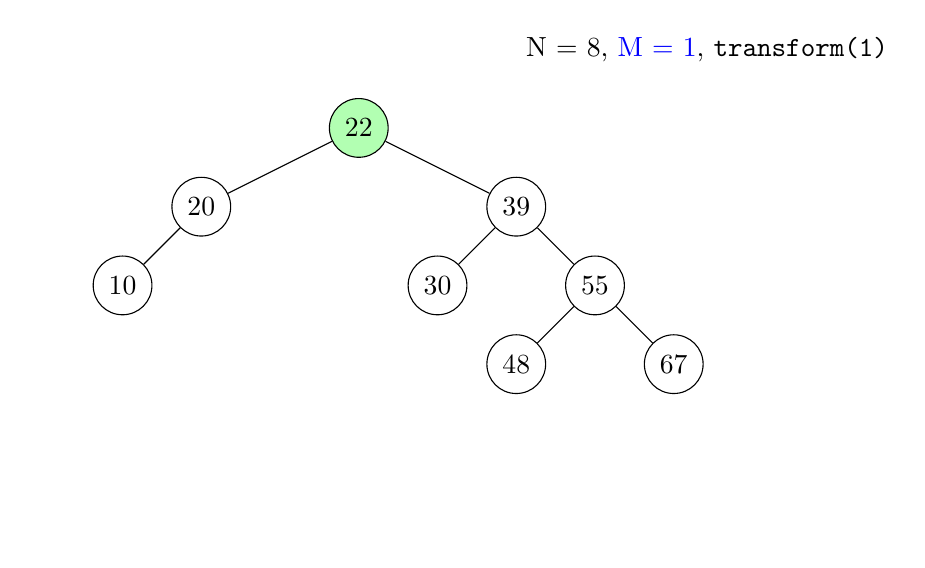
\begin{tikzpicture}
        \begin{scope}{shift={(3,0)}}
            \node[opacity=0] (X) at (1, 2) { $1$ };
            \node[circle,draw] (A) at (3, 6) { 20 };
            \node[circle,draw] (B) at (2, 5) { 10 };
            \node[circle,draw] (C) at (7, 4) { 48 };
            \node[circle,draw] (D) at (6, 5) { 30 };
            \node[circle,draw] (E) at (8, 5) { 55 };
            \node[circle,draw,fill=green!30] (F) at (5, 7) { 22 };
            \node[circle,draw] (G) at (7, 6) { 39 };
            \node[circle,draw] (H) at (9, 4) { 67 };

            \draw (A) -- (B);
            \draw (A) -- (F);
            \draw (C) -- (E);
            \draw (F) -- (G);
            \draw (D) -- (G);
            \draw (E) -- (G);
            \draw (E) -- (H);

            \node[anchor=west] at (7, 8) { N = 8, \textcolor{blue}{M = 1}, \texttt{transform(1)} };
        \end{scope}
    \end{tikzpicture}

\end{frame}

\begin{frame}
\frametitle{Algoritmo DSW: transformação da espinha dorsal}

    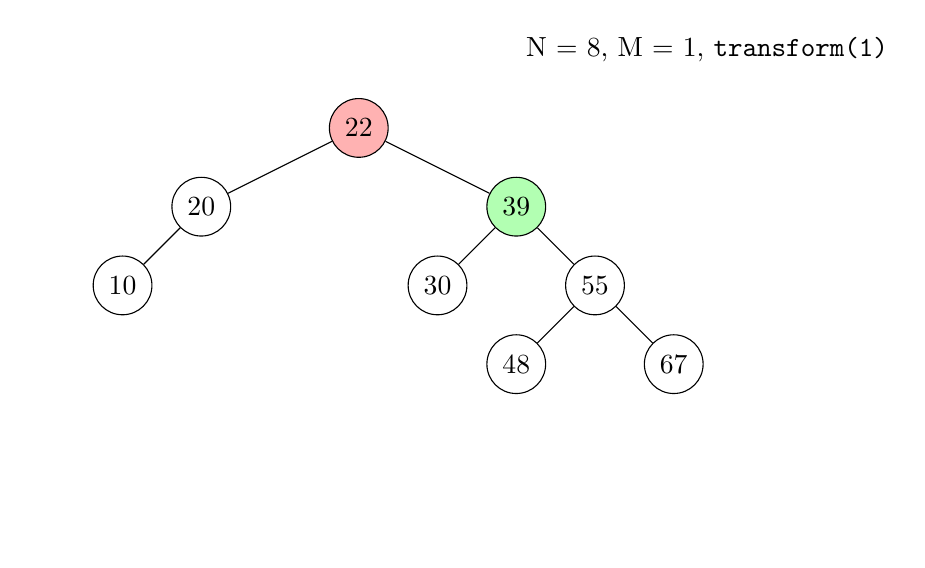
\begin{tikzpicture}
        \begin{scope}{shift={(3,0)}}
            \node[opacity=0] (X) at (1, 2) { $1$ };
            \node[circle,draw] (A) at (3, 6) { 20 };
            \node[circle,draw] (B) at (2, 5) { 10 };
            \node[circle,draw] (C) at (7, 4) { 48 };
            \node[circle,draw] (D) at (6, 5) { 30 };
            \node[circle,draw] (E) at (8, 5) { 55 };
            \node[circle,draw,fill=red!30] (F) at (5, 7) { 22 };
            \node[circle,draw,fill=green!30] (G) at (7, 6) { 39 };
            \node[circle,draw] (H) at (9, 4) { 67 };

            \draw (A) -- (B);
            \draw (A) -- (F);
            \draw (C) -- (E);
            \draw (F) -- (G);
            \draw (D) -- (G);
            \draw (E) -- (G);
            \draw (E) -- (H);

            \node[anchor=west] at (7, 8) { N = 8, \textcolor{black}{M = 1}, \texttt{transform(1)} };
        \end{scope}
    \end{tikzpicture}

\end{frame}

\begin{frame}
\frametitle{Algoritmo DSW: transformação da espinha dorsal}

    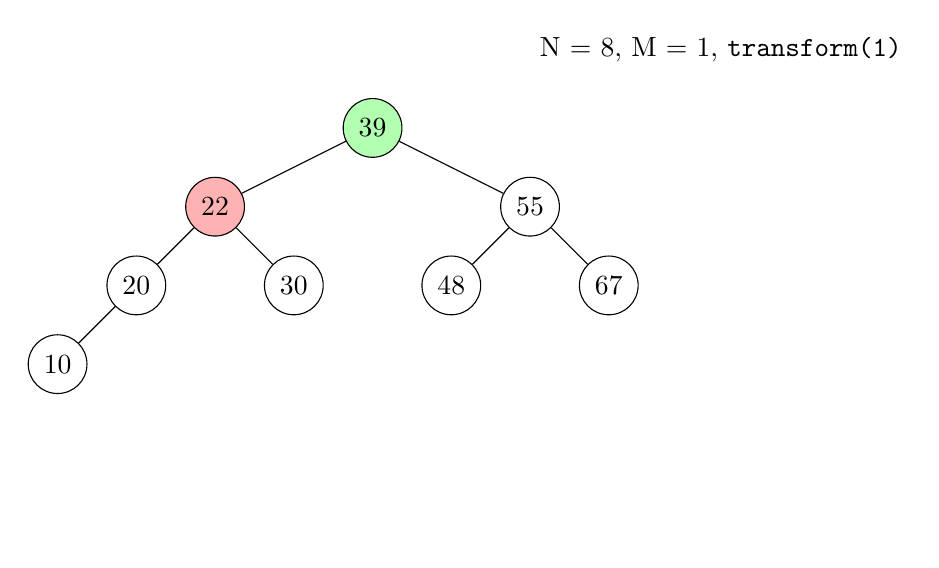
\begin{tikzpicture}
        \begin{scope}{shift={(3,0)}}
            \node[opacity=0] (X) at (1, 2) { $1$ };
            \node[circle,draw] (A) at (2, 5) { 20 };
            \node[circle,draw] (B) at (1, 4) { 10 };
            \node[circle,draw] (C) at (6, 5) { 48 };
            \node[circle,draw] (D) at (4, 5) { 30 };
            \node[circle,draw] (E) at (7, 6) { 55 };
            \node[circle,draw,fill=red!30] (F) at (3, 6) { 22 };
            \node[circle,draw,fill=green!30] (G) at (5, 7) { 39 };
            \node[circle,draw] (H) at (8, 5) { 67 };

            \draw (A) -- (B);
            \draw (A) -- (F);
            \draw (C) -- (E);
            \draw (F) -- (G);
            \draw (D) -- (F);
            \draw (E) -- (G);
            \draw (E) -- (H);

            \node[anchor=west] at (7, 8) { N = 8, \textcolor{black}{M = 1}, \texttt{transform(1)} };
        \end{scope}
    \end{tikzpicture}

\end{frame}
